\section{Auswertung}%
\label{sec:auswertung}
4a,j
4b
4d, 4e
4f
4g
4h
\subsection{Linearverst\"arker}
Der Verstärkungsfaktor $V$ wird gegen die Frequenz $\nu$ in einem doppellogarithmischen Diagramm aufgetragen.
Es wird ein ein Fit für Tiefpässe berechnet, nach Gleichung~\eqref{eq:h_betrag}:
\begin{equation}
  V = \frac{V'}{\sqrt{1 + {\left(\nu RC\right)}^{2}}}
\end{equation}
Die Messwerte sind mit dem Fit in den Abbildungen~\ref{fig:lin_verst_01} bis~\ref{fig:lin_verst_04} dargestellt.
Die vier verschiedenen Konfigurationen sind in den Abbildungsunterschriften zu finden,
die Grenzfrequenz $\nu_\text{G} = RC$ in der entsprechenden Legende.

\begin{figure}[ht]
  \centering
  \input{build/lin_verst_01__r1_200__rn_470__u1_100.pgf}
  \caption{Linearer Verst\"arker mit $R_1 = \SI{200}{\kilo\ohm}$, $R_N = \SI{470}{\kilo\ohm}$.}
  \label{fig:lin_verst_01}
\end{figure}

\begin{figure}[ht]
  \centering
  \input{build/lin_verst_02__r1_200__rn_100__u1_100.pgf}
  \caption{Linearer Verst\"arker mit $R_1 = \SI{200}{\kilo\ohm}$, $R_N = \SI{100}{\kilo\ohm}$}
  \label{fig:lin_verst_02}
\end{figure}

\begin{figure}[ht]
  \centering
  \input{build/lin_verst_03__r1_100__rn_470__u1_100.pgf}
  \caption{Linearer Verst\"arker mit $R_1 = \SI{100}{\kilo\ohm}$, $R_N = \SI{470}{\kilo\ohm}$}
  \label{fig:lin_verst_03}
\end{figure}

\begin{figure}[ht]
  \centering
  \input{build/lin_verst_04__r1_470__rn_100__u1_100.pgf}
  \caption{Linearer Verst\"arker mit $R_1 = \SI{470}{\kilo\ohm}$, $R_N = \SI{100}{\kilo\ohm}$}
  \label{fig:lin_verst_04}
\end{figure}

Die Abweichung des Verstärkungsfaktors aus dem Fit mit dem Verhältnis $\sfrac{R_N}{R_1}$
sind
\begin{align*}
  \Delta V_{\ref{fig:lin_verst_01}} &= \num{3.444}\% \\
  \Delta V_{\ref{fig:lin_verst_02}} &= \num{4.417}\% \\
  \Delta V_{\ref{fig:lin_verst_03}} &= \num{0.118}\% \\
  \Delta V_{\ref{fig:lin_verst_04}} &= \num{1.536}\%.
\end{align*}
Die aus Gleichung~\eqref{eq:v_strich} bestimmten Leerlaufverstärkungen sind
\begin{align*}
  V_{\ref{fig:lin_verst_01}} &= \num{65.88} \\
  V_{\ref{fig:lin_verst_02}} &= \num{10.82} \\
  V_{\ref{fig:lin_verst_03}} &= \num{-4002.54} \\
  V_{\ref{fig:lin_verst_04}} &= \num{-14.06}.
\end{align*}

Es werden die Phasendifferenzen zwischen Ein- und Ausgangsspannung gegen die Frequenz
in einem halblogarithmischen Diagramm in Abbildung~\ref{fig:phasendiff} aufgetragen.

\begin{figure}[ht]
  \centering
  \input{build/phases.pgf}
  \caption{Phasendifferenz der Ein- und Ausgangsspannung aller Verstärker.}
  \label{fig:phasendiff}
\end{figure}

\subsection{Umkehrintegrator}
\begin{figure}[ht]
  \centering
  \input{build/integrator.pgf}
  \caption{}
  \label{fig:int}
\end{figure}
\begin{figure}[ht]
  \centering
  \begin{subfigure}[]{\textwidth}
    \centering
    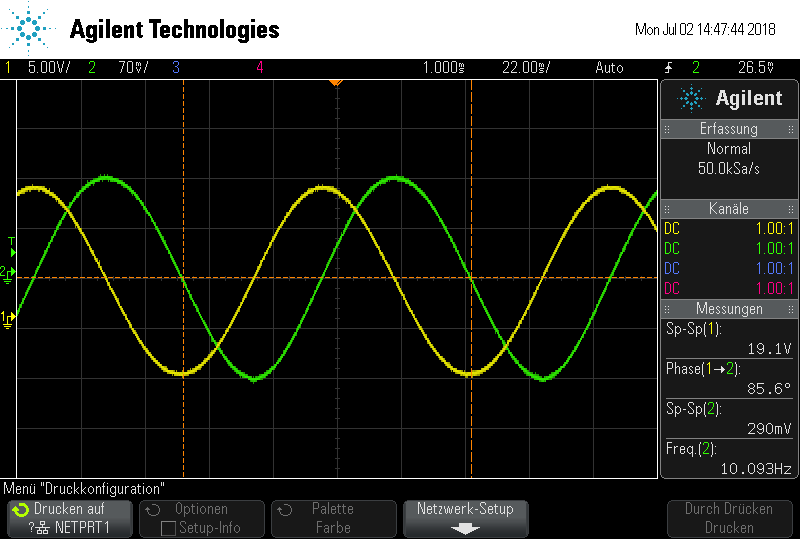
\includegraphics[height=0.3\textheight]{data/scope_262.png}
    \caption{Integration einer Sinusspannung.}
    \label{subfig:int_sinus}
  \end{subfigure}
  \begin{subfigure}[]{\textwidth}
    \centering
    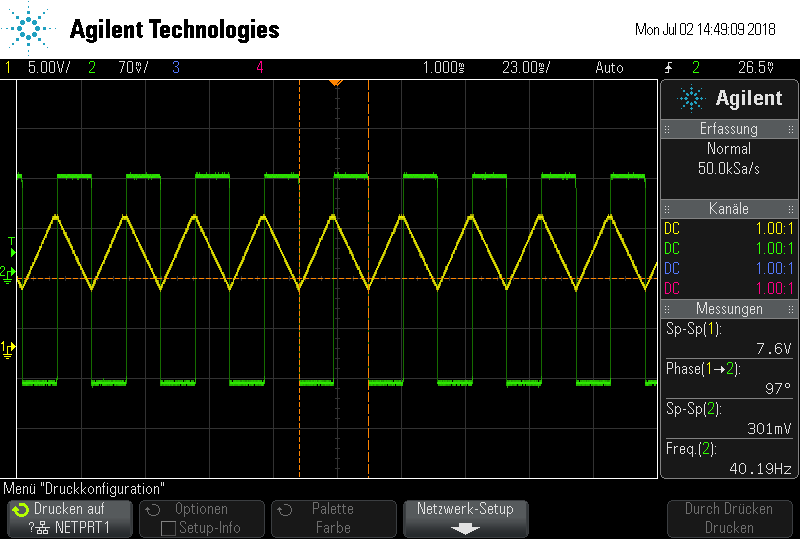
\includegraphics[height=0.3\textheight]{data/scope_263.png}
    \caption{Integration einer Rechteckspannung.}
    \label{subfig:int_rechteck}
  \end{subfigure}
  \begin{subfigure}[]{\textwidth}
    \centering
    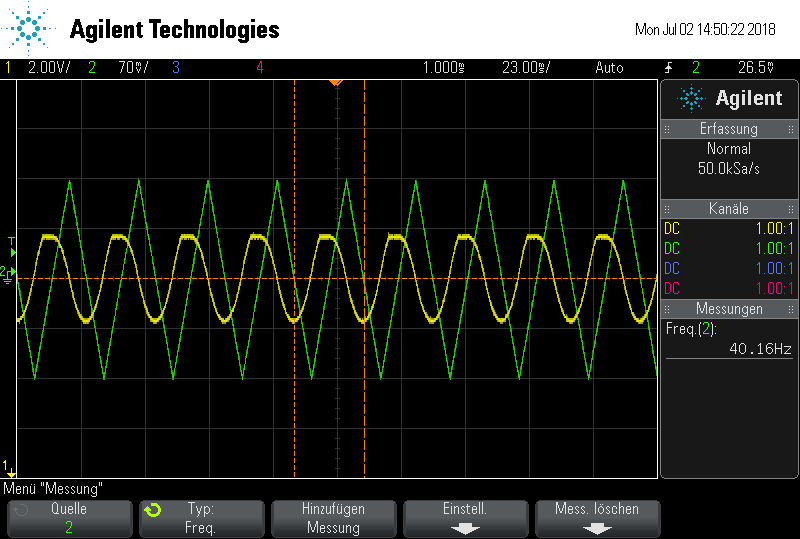
\includegraphics[height=0.3\textheight]{data/scope_264.png}
    \caption{Integration einer Dreieckspannung.}
    \label{subfig:int_dreieck}
  \end{subfigure}
  \caption{Aufnahmen des Oszilloskops von verschiedenen Integrationen.}
  \label{fig:integrationen}
\end{figure}

\subsection{Umkehrdifferentiator}
\begin{figure}[ht]
  \centering
  \input{build/differentiator.pgf}
  \caption{}
  \label{fig:dif}
\end{figure}
\begin{figure}[ht]
  \centering
  \begin{subfigure}[]{\textwidth}
    \centering
    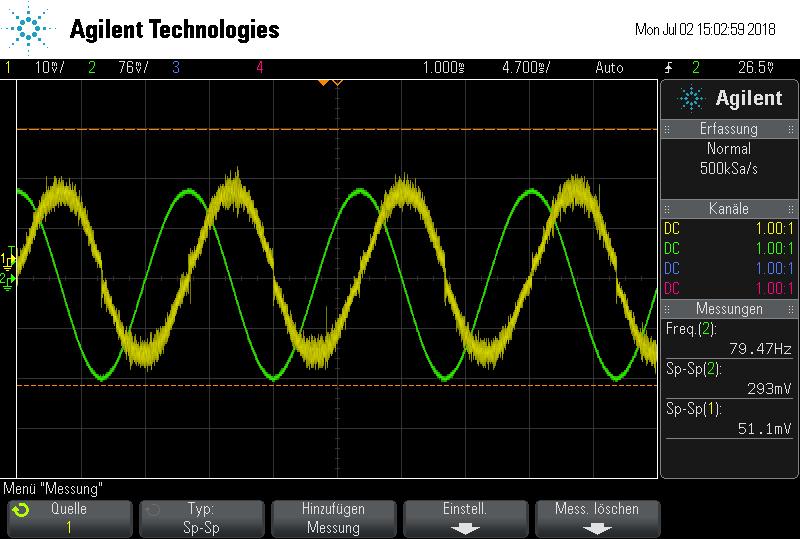
\includegraphics[height=0.3\textheight]{data/scope_265.png}
    \caption{Differentiation einer Sinusspannung.}
    \label{subfig:dif_sinus}
  \end{subfigure}
  \begin{subfigure}[]{\textwidth}
    \centering
    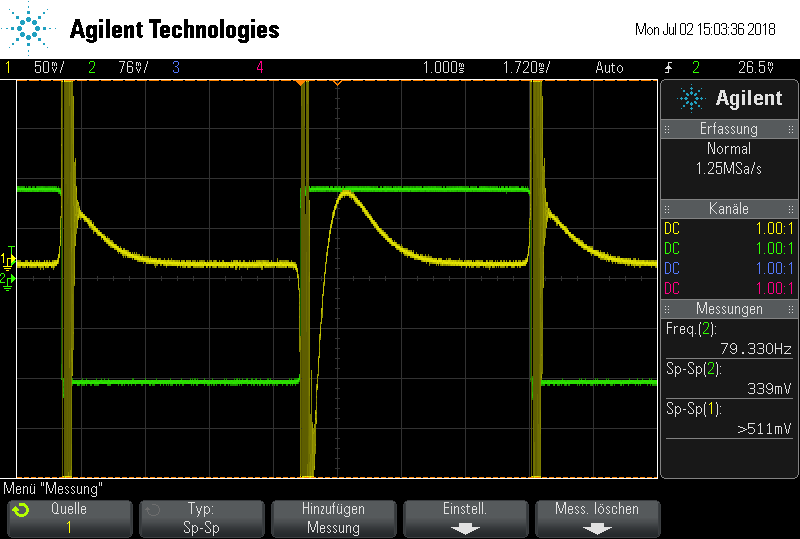
\includegraphics[height=0.3\textheight]{data/scope_266.png}
    \caption{Differentiation einer Rechteckspannung.}
    \label{subfig:dif_rechteck}
  \end{subfigure}
  \begin{subfigure}[]{\textwidth}
    \centering
    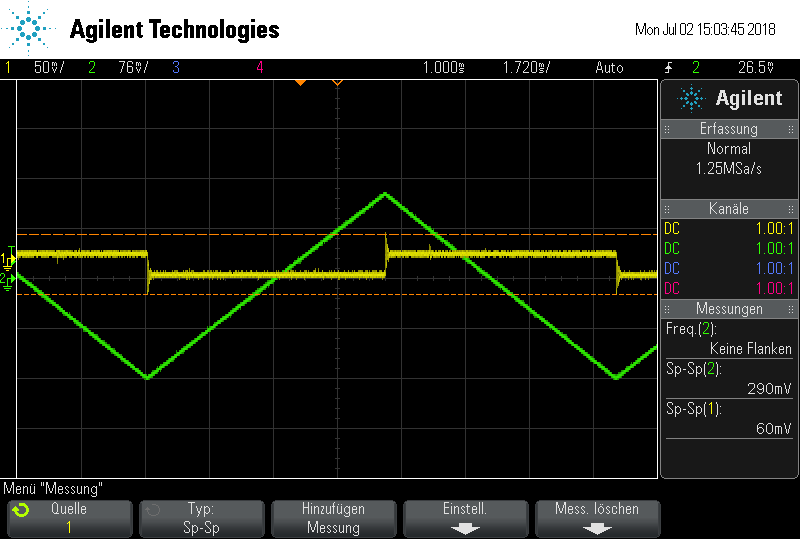
\includegraphics[height=0.3\textheight]{data/scope_267.png}
    \caption{Differentiation einer Dreieckspannung.}
    \label{subfig:dif_dreieck}
  \end{subfigure}
  \caption{Aufnahmen des Oszilloskops von verschiedenen Differentiationen.}
  \label{fig:integrationen}
\end{figure}

\subsection{Schmitt-Trigger}
\begin{figure}[ht]
  \centering
  \begin{subfigure}{\textwidth}
    \centering
    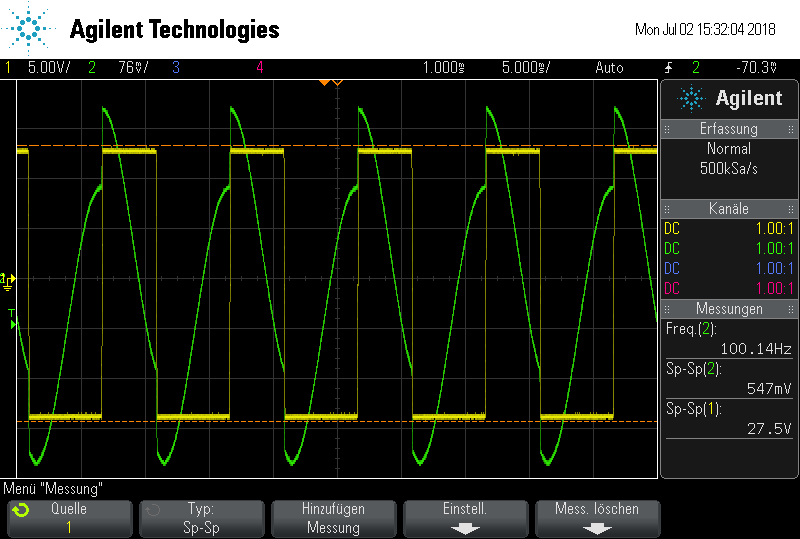
\includegraphics[height=0.3\textheight]{data/scope_268.png}
    \caption{Aufnahmen des Oszilloskops.}
    \label{fig:schmitt_osz}
  \end{subfigure}
  \begin{subfigure}{\textwidth}
    \centering
    \input{build/schmitt.pgf}
    \caption{Oszilloskopdaten mit markierter Schwelle der Sinuseingangsspannung.}
    \label{fig:schmitt_plot}
  \end{subfigure}
  \caption{Name}
  \label{fig:schmitt}
\end{figure}

\subsection{Dreieckgenerator}
\begin{figure}[ht]
  \centering
  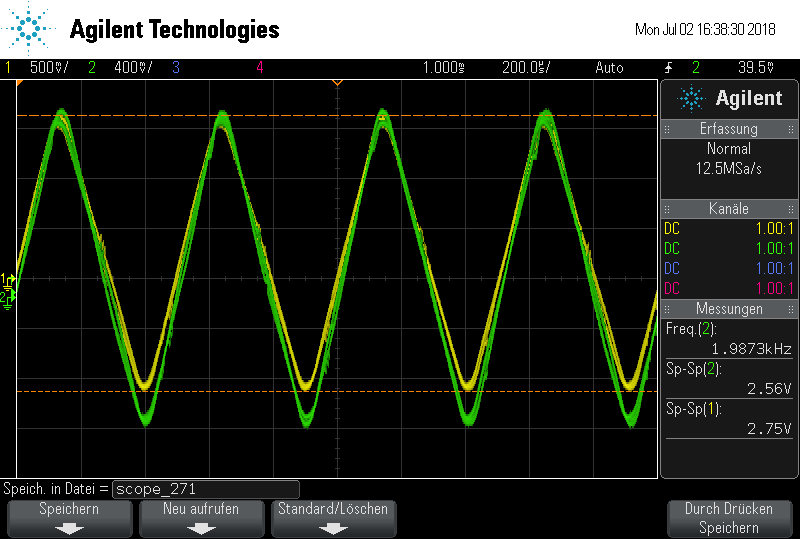
\includegraphics[height=0.3\textheight]{data/scope_271.png}
  \caption{Name}
  \label{fig:dreieck_generator}
\end{figure}

\subsection{Ged\"ampfte Schwingung}
\begin{figure}[ht]
  \centering
  \begin{subfigure}{\textwidth}
    \centering
    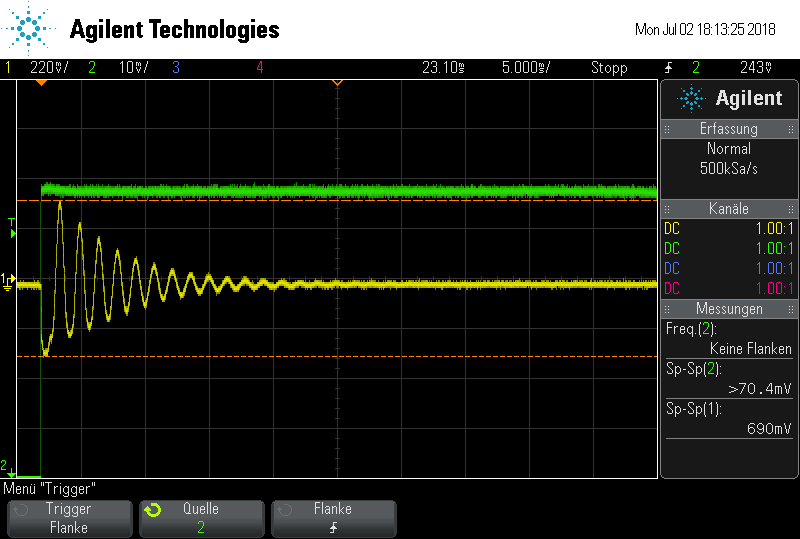
\includegraphics[height=0.3\textheight]{data/scope_275.png}
    \caption{Aufnahmen des Oszilloskops.}
    \label{fig:}
  \end{subfigure}
  \begin{subfigure}{\textwidth}
    \centering
    \input{build/gedaempfte_schwingung.pgf}
    \caption{Oszilloskopdaten mit Fit.}
    \label{fig:}
  \end{subfigure}
  \caption{Name}
  \label{fig:gedaempft}
\end{figure}
